\documentclass[a4paper,fleqn]{cas-dc}

% If the frontmatter runs over more than one page
% use the longmktitle option.

%\documentclass[a4paper,fleqn,longmktitle]{cas-sc}

\usepackage[numbers]{natbib}
%\usepackage[authoryear]{natbib}
%\usepackage[authoryear,longnamesfirst,square]{natbib}
%\usepackage{soul}

% user defined package
\usepackage{setspace}
\usepackage[version=4]{mhchem}
% user defined package

%%%Author macros
\def\tsc#1{\csdef{#1}{\textsc{\lowercase{#1}}\xspace}}
\tsc{WGM}
\tsc{QE}
%%%

\newcommand{\zd}[1]{\textcolor{brown}{{\sffamily ZD:  #1}}}
\def\tm#1{\textcolor[rgb]{0,0,1}{{\sffamily TMP:  #1}}}
\newcommand{\pc}[1]{\textcolor{teal}{{\sffamily PC: #1}}}
\newcommand{\sai}[1]{\textcolor{orange}{{\sffamily GSG: #1}}}
\def\wx#1{\textcolor[rgb]{1,0,1}{{\sffamily WX:  #1}}}


% Uncomment and use as if needed
%\newtheorem{theorem}{Theorem}
%\newtheorem{lemma}[theorem]{Lemma}
%\newdefinition{rmk}{Remark}
%\newproof{pf}{Proof}
%\newproof{pot}{Proof of Theorem \ref{thm}}
\begin{document}
\let\WriteBookmarks\relax
\def\floatpagepagefraction{1}
\def\textpagefraction{.001}

% Short title
\shorttitle{\texttt{kMCpy}: A Python Package to Simulate Transport Properties in Solids with Kinetic Monte Carlo}    

% Short author
\shortauthors{Zeyu Deng, Tara P. Mishra,  Weihang Xie, and Pieremanuele Canepa}  

% Main title of the paper
\title [mode = title]{\texttt{kMCpy}:  A Python Package to Simulate Transport Properties in Solids with Kinetic Monte Carlo}  

% Title footnote mark
% eg: \tnotemark[1]
%\tnotemark[<tnote number>] 

% Title footnote 1.
% eg: \tnotetext[1]{Title footnote text}
%\tnotetext[<tnote number>]{<tnote text>} 

% First author
%
% Options: Use if required
% eg: \author[1,3]{Author Name}[type=editor,
%       style=chinese,
%       auid=000,
%       bioid=1,
%       prefix=Sir,
%       orcid=0000-0000-0000-0000,
%       facebook=<facebook id>,
%       twitter=<twitter id>,
%       linkedin=<linkedin id>,
%       gplus=<gplus id>]


\author[1]{Zeyu Deng}[
prefix=Dr.,
orcid=0000-0003-0109-9367
]
\credit{Conceptualization of the study, Methodology, Software development, Writing the Initial Draft}
\ead{msedz@nus.edu.sg}
\cormark[1]
\cortext[1]{Corresponding author.}

\author[1,2]{Tara P. Mishra}[
prefix=Dr.,
orcid=0000-0002-3000-2555
]
\credit{Software development, Writing the Initial Draft}

\author[1]{Weihang Xie}[
prefix=Mr.,
orcid=0000-0002-6498-2328
]
\credit{Software development, Writing the Initial Draft}
\author[5]{Daanyal Ahmed Saeed}[
prefix=Mr.,
orcid=0000-0003-4620-4829
]
\credit{Software development, Writing the Initial Draft}
\author[3]{Gopalakrishnan Sai Gautam}[
prefix=Prof.,
orcid=0000-0002-1303-0976
]
\credit{Methodology, Writing the Initial Draft}

\author[1,2,4]{Pieremanuele Canepa}[
prefix=Prof.,
orcid=0000-0002-5168-9253
]
\ead{pcanepa@nus.edu.sg}
\credit{Conceptualization of the study, Methodology, Project Management, Procurement of Funding, Writing the Initial Draft}
% Corresponding author indication
\cormark[1]



% Credit authorship
% eg: \credit{Conceptualization of this study, Methodology, Software}


% Address/affiliation
\affiliation[1]{
            organization=National University of Singapore,
            addressline={Department of Materials Science and Engineering, 9 Engineering Drive 1}, 
            city={Singapore},
            citysep={}, % Uncomment if no comma needed between city and postcode
            postcode={117575}, 
            country={Singapore}}

% Footnote of the second author
%\fnmark[2]
\affiliation[2]{
            organization={Singapore-MIT Alliance for Research and Technology},
            addressline={1 CREATE Way, 10-01 CREATE Tower}, 
            city={Singapore},
            citysep={}, % Uncomment if no comma needed between city and postcode
            postcode={138602}, 
            country={Singapore}
            }

\affiliation[3]{
            organization={Indian Institute of Science},
            addressline={Department of Materials Engineering, Indian Institute of Science}, 
            city={Bengaluru},
            citysep={}, % Uncomment if no comma needed between city and postcode
            postcode={560012}, 
            country={India}
            }
            
% Address/affiliation
\affiliation[4]{
            organization={National University of Singapore},
            addressline={Department of Chemical and Biomolecular Engineering, 4 Engineering Drive 4}, 
            city={Singapore},
            citysep={}, % Uncomment if no comma needed between city and postcode
            postcode={117585}, 
            country={Singapore}
            }
\affiliation[5]{
            organization={University of California, Berkeley},
            addressline={2437 Piedmont Avenue}, 
            city={Berkeley, California},
            citysep={}, % Uncomment if no comma needed between city and postcode
            postcode={94704}, 
            country={United States of America}
            }
            
% Corresponding author text


% Footnote text
%\fntext[1]{test}

% For a title note without a number/mark
%\nonumnote{}

% Here goes the abstract
\begin{abstract}
Understanding ion transport in functional materials is crucial to unravel complex chemical reactions, improve rate performance of materials for energy storage and conversion, and optimize catalysts. To model ionic transport, atomistic simulations, including molecular dynamics (MD) and kinetic Monte Carlo (kMC) have been developed and applied to shed light on intricate materials science and chemistry problems. Typically, kMC simulations are utilized to a lower extent compared to MD due to a lack of systematic workflows to construct a model for predicting transition rates. Here, we propose \texttt{kMCpy}, a light-weight, customizable, and modular \texttt{python} package to compute the ionic transport properties in crystalline materials using kMC that can be combined with a (local) cluster expansion Hamiltonian derived from first-principles calculations. \texttt{kMCpy} is versatile with respect to any type of crystalline material, bearing any dimensionality, such as 1D, 2D and 3D. \texttt{kMCpy} provides: i) a comprehensive workflow to enumerate all possible migration events in crystalline systems, ii) to derive transition rates efficiently and at the accuracy of first-principles calculations, and iii) a robust kMC solver to study kinetic phenomena in materials.  The workflow implemented in \texttt{kMCpy} provides a systematic way to compute highly-accurate kinetic properties, which can be used in high-throughput simulations for the discovery and optimization of novel functional materials.
\end{abstract}

% Use if graphical abstract is present
%\begin{graphicalabstract}
%\includegraphics{}
%\end{graphicalabstract}

% Research highlights
\begin{highlights}
    \item Kinetic Monte Carlo
\end{highlights}

% Keywords
% Each keyword is seperated by \sep
\begin{keywords}
Kinetic Monte Carlo \sep Transport Property \sep Kinetics \sep Cluster Expansion \sep Ion Transport
\end{keywords}


\maketitle

% Main text
% user defined package
% \onehalfspacing
% user defined package
\section{Introduction}\label{sec:intro}
\noindent Quantifying ionic transport properties in materials is crucial in a wide variety of applications, such as molecular \& protein biology\cite{mccammon_dynamics_1977,karplus_molecular_2005,klepeis_long-timescale_2009}, energy\cite{ong_electrochemical_2011,mo_insights_2014,wang_design_2015}, chemical reactions\cite{herschbach_molecular_1987,craig_chemical_2005}, and solid mechanics.\cite{lutsko_stress_1988,abraham_molecular_1997,yang_multiscale_2006,rafii-tabar_molecular_2006} The advancement of computer hardware, theoretical models, and suitable software that scale and parallelize with available computing resources, have  enabled the evaluation of ionic transport in solid-state materials.\cite{frenkel_understanding_2002,balluffi_kinetics_2005} A widely used atomistic simulation technique to probe kinetic properties is molecular dynamics (MD),\cite{frenkel_understanding_2002,hansson_molecular_2002} which propagates the state of a given system as a function of time, where individual particles (atoms) interact via Newton's laws of motion. MD has been implemented in a wide variety of software packages\cite{thompson_lammps_2022,te_velde_chemistry_2001,phillips_scalable_2020,apra_nwchem_2020,salomon-ferrer_overview_2013,kuhne_cp2k_2020}, where the accuracy of MD is dependent on the accuracy of force evaluations. Forces acting on atoms in a MD simulation is accessed from accurate (but expensive) first principles calculations, or inexpensive (and less accurate) interatomic potentials (i.e., force fields).

An alternative to MD is kinetic Monte Carlo (kMC, also known as dynamic Monte Carlo)\cite{bortz_new_1975,gillespie_general_1976,gillespie_exact_1977}, which has  been extensively applied to study materials kinetics including, rechargeable batteries\cite{van_der_ven_first-principles_2001,van_der_ven_rechargeable_2020,xiao_kinetic_2018,deng_fundamental_2022}, solid-oxide fuel cells\cite{pornprasertsuk_kinetic_2009,modak_kinetic_2005},  catalysis\cite{Andersen2019,pineda_kinetic_2022}, crystal growth\cite{huang_mechanism_2017},  vacancy diffusion in alloys\cite{evteev_shrinking_2008,li_predicting_2021}, thin film growth\cite{han_development_2007}, and fluid flow\cite{apostolopoulou_kinetic_2017}. kMC is particularly useful in quantifying ionic transport in battery materials, as demonstrated by van der Ven \textit{et al.} in electrode materials, such as \ce{Li_xCoO2}\cite{van_der_ven_first-principles_2001}, \ce{Li_xTiS2}\cite{van_der_ven_nondilute_2008}, \ce{Li_{1+x}Ti2O4}\cite{bhattacharya_phase_2010}.  Notably, Deng \textit{et al.}\cite{deng_fundamental_2022} used kMC to estimate the conductivity of Na in solid electrolytes: \ce{Na_{1+x}Zr_2P_x Si_{3-x}O_{12}}, as a function of Na content and temperature, eventually sampling a vast compositional, spatial, and temporal scale. kMC can also be used to examine the structural evolution of nano-particles as well, as demonstrated by Li \textit{et al.}{\cite{li_predicting_2021}}.

kMC is based on a stochastic algorithm which randomly samples various microstates of a given system, utilizing the ergodic principle to arrive at statistically-averaged transport properties. Thus, the chief advantage of kMC over MD is the ability of kMC to access ``long'' timescales ($\sim$ms) and ``large'' lengthscales ($\sim\mu$m) compared to what is usually possible in MD ($\sim\mu$s, $\sim$nm)\cite{gao_design_2022}.

Two main kMC algorithms have been proposed: i) kMC with rejection (r-kMC)\cite{hastings_monte_1970} and ii) rejection-free kMC (rf-kMC)\cite{bortz_new_1975}. The former algorithm is similar to the Metropolis algorithm\cite{hastings_monte_1970} which can select or reject a transition event using a probability estimate. In rf-kMC, a transition event is always executed based on a ``list'' of probabilities. Thus, rf-kMC is computationally efficient compared to r-kMC, especially when transition rates are low (i.e., event rejection rates are high). There are several software packages to perform kMC simulations \cite{magna_lattice_1999,dooling_generic_2001,boerrigter_monty_2004,leetmaa_kmclib_2014,Hoffmann2014a,ramsey_james_j_kmcthinfilm_2015,mitchell_global_2016,danielson_sqertss_2017,jorgensen_montecoffee_2018,li_crystal-kmc_2018,li_openkmc_2019,martin_kimera_2020}, including codes that target higher efficiency kMC algorithms\cite{schulze_kinetic_2002,bernacki_multiple_2004,shi_parallel_2007,xu_adaptive_2008,slepoy_constant-time_2008,chatterjee_accurate_2010,nielsen_parallel_2013}, and those that construct novel models to compute accurate transition rates\cite{xu_simulating_2011,konwar_off-lattice_2011,stamatakis_graph-theoretical_2011,guo_--fly_2015,yang_learning_2017}.

Compared to MD, kMC is a fairly general simulation algorithm which can be applied to coarse grain material properties and contribute to multi scale modelling efforts\cite{chatterjee_multiscale_2006,collins_coarse-grained_2008,deng_towards_2022}. However, in kMC all transition events should be known \emph{a priori}, and a model is typically needed to compute transition rates between different microstates swiftly. Therefore, using kMC to study ionic transport usually needs a workflow that is typically ``tailored'' to a given system. Such a workflow should include  modules to generate all possible transition events, a comprehensive model to compute transition rate for each event (swiftly and accurately), and a robust kMC solver.

Here, we present our \texttt{python}-based code \texttt{kMCpy}\footnote{\texttt{kMCpy} is an open-source code developed under the MIT license and can be accessed at: https://github.com/caneparesearch/kMCpy\label{fn:github}} to simulate the kinetic properties of materials, with inputs from first principles calculations. Specifically, we implement a local cluster expansion (LCE) model\cite{van_der_ven_first-principles_2001,van_der_ven_rechargeable_2020} to compute migration barriers in crystalline materials (within the transition state theory framework), where the model is fitted to calculated barriers from accurate first principles calculations. \texttt{kMCpy} contains a rf-kMC solver and related \texttt{python} classes to extract ion transport properties, such as diffusivities, conductivities, etc. In addition, \texttt{kMCpy} includes the following features:
\begin{itemize}
    \item \texttt{kMCpy} is fully developed using \texttt{python}\cite{perez_python_2011,noauthor_top_2022}.
    \item Cross Platform: \texttt{kMCpy} supports most ``mainstream'' operating systems, such as Windows, macOS, and Linux, in both x86/64 and ARM architectures.
    \item Modular Code Structure: \texttt{kMCpy} is written as modulus, which can be easily modified and ported to any specific application. 
    \item Ease of Use: All input and output data are supplied using human-readable JSON format, which is easily parsed and generated by computers.
    \item Performance: The computationally-intensive routines  of \texttt{kMCpy} are translated into optimized machine code at runtime using \texttt{Numba} \cite{lam_numba_2015}, which is a just-in-time (JIT) compiler desgined to  increase computational performance of \texttt{python} codes.
\end{itemize}

The paper is structured as follows: Sec.~{\ref{sec:theory}} deals with the theoretical background to compute transport properties in crystalline materials, Sec.~{\ref{sec:code}} provides an overview of the \texttt{kMCpy} code,  Sec.~\ref{sec:performance} describes the performance of \texttt{kMCpy}, and Sec.~{\ref{sec:conclusion}} compiles our concluding remarks and possible future developments of \texttt{kMCpy}. All nomenclature used through the manuscript is listed in Sec.~\ref{sec:nomenclature}.  

%% The Appendices part is started with the command \appendix;
%% appendix sections are then done as normal sections
%% \appendix
\section{Theoretical Background}\label{sec:theory}

\noindent Ionic transport in solids is a stochastic process, occurring through a series of correlated/non-correlated migration events (or ionic 'hops'), which can be effectively modeled using the kMC formalism. The local energy landscape around the migrating ion determines the ease of migration within the solid. Quantifying macroscopic ionic transport of a given chemical species in a given material is usually done in terms of ionic diffusivities and/or ionic conductivities (see below), both of which can be evaluated using kMC.\cite{van_der_ven_first-principles_2001}  

Before understanding how a typical kMC simulation progresses, we briefly overview some of the fundamentals of ion transport in solids. The macroscopic measure of  mobility of a migrating species is determined by the chemical diffusivity ($D_{c}$), which relates to the flux and conductivity of the species through Fick's law\cite{fick_v_1855,fick_ueber_1855}, as stated in Eq.~{\ref{eq:flux}.} 
%
\begin{equation}
    \label{eq:flux}
    J= -D_{c} \nabla C
\end{equation}
%
where $J$ is the flux of the migrating species, and C is the composition of the mobile species defined as the number of migrating ions per unit volume. The chemical diffusivity of the migrating ion relates to the jump diffusivity ($D_J$) through the thermodynamic factor $\Theta$ of  Eq.~{\ref{eq:jumpdiff}}.
%
\begin{equation}
\label{eq:jumpdiff}
D_{c} = D_{J} \Theta
\end{equation}
%
$\Theta$ measures the deviation of the interaction between migrating ions from ideal behavior and is given in Eq.~\ref{eq:thermodynamic_factor}
%
\begin{equation}
\label{eq:thermodynamic_factor}
\Theta = \frac{\partial \left(\frac{\mu}{k_B T}\right)}{\partial \ln{x}}
\end{equation}
%
where $\mu$ is the chemical potential, $k_B$ is the Boltzmann constant, and $x$ is the molefraction of the migrating species. 

$D_J$ of Eq.~\ref{eq:jumpdiff} is proportional to the mean squared displacement of the center of mass of the mobile species, as mathematically described in Eq.~\ref{eq:jumpdiff_atomistic}.
%
\begin{equation}
\label{eq:jumpdiff_atomistic}
D_J = \frac{\left(\sum_i \vec{r_i}\right)^2}{2dNt}
\end{equation}
%
where $d$ is the dimensionality of the diffusion process, $N$ is the number of diffusing species, and $t$ is the time taken for diffusion. Furthermore, from the square of displacements of the migrating ions, one can also calculate the tracer diffusivity ($D^{*}$, Eq.~\ref{eq:tracerdiff_atomistic}), which excludes cross-correlation effects between the migrating ion \cite{van_der_ven_rechargeable_2020}.
%
\begin{equation}
\label{eq:tracerdiff_atomistic}
D^{*} = \frac{\sum_i \vec{r_i}^2}{2dNt} 
\end{equation}
%
The ionic conductivity $\sigma$ can be then computed via the Nernst–Einstein relationship:
%
\begin{equation}
    \label{eq:conduct}
    \sigma=\frac{e^2CD_J}{k_BT}
\end{equation}
%
{where $C$ is the number of migrating species per unit volume.

Therefore, the cross-correlation between migrating ions  can be quantified from the ratio of $D^{*}$ and $D_{J}$, which is called the Haven's ratio ($H_R$) \cite{murch_haven_1982}. Note that H$_R$ does not measure the correlation between subsequent hops of a single ion that is migrating, i.e., the deviation of the trajectory of a single migrating ion from a fully random walk. This deviation from a fully random walk is measured by the correlation factor ($f$) of Eq.~\ref{eq:correlation_factor}.
%
\begin{equation}
    \label{eq:correlation_factor}
    f = \frac{\sum_i \vec{r_i}^2}{Nna^2}
\end{equation}
%
where $\vec{r_i}$ is the net displacement of a migrating ion after $n$ hops, while $a$ is the average distance for a single hop. Therefore, an accurate calculation of the ionic transport properties requires the sampling of a large-enough number of migration events, which requires  that all mobile species are tracked during the simulation.

One of the important parameters required by a kMC simulation are the migration barriers ($E_{b}$s), which are the energy barrierers that the mobile ion must  overcome to complete a successful hop. $E_b$ ultimately determines the probability of occurrence a given ionic hop. Typically, $E_b$s are evaluated using the nudged elastic band (NEB) method in combination with density functional theory (DFT). \cite{jonsson_nudged_1998,henkelman_climbing_2000}. In a NEB calculation, one performs a constrained relaxation  of a specific number of virtually connected ``images'', between the initial and final positions of a migration event, along a guessed minimum energy pathway (MEP). The relaxation is constrained to maintain a uniform spacing between the images (i.e., as uniform as possible), through the addition of fictitious spring forces. Other tools, such as force fields and machine-learned interatomic potentials, can also be used to determine $E_b$ instead of DFT, and \texttt{kMCpy} is also compatible with such tools.

Note that $E_b$ in solids not only depends on the local environment of the migrating ion but also the  direction of the hop. Hence, to remove any direction-dependence of a hop, we resort to the so-called kinetically resolved activation barrier ($E_\mathrm{KRA}$) of Eq.~\ref{eq:ekra} proposed by van der Ven et al. \cite{van_der_ven_first-principles_2001}.
%
\begin{equation}
    \label{eq:ekra}
    E_\mathrm{KRA} = E_{b} [i \rightarrow j] -\frac{1}{2} \Delta E_\mathrm{end}
\end{equation}
%
where $E_{b} [i \rightarrow j]$ is the calculated $E_b$ (e.g., with NEB) for a site $i$ to site $j$ hop and $\Delta E_{\mathrm{end}}$ is the absolute difference between the computed DFT total energies of the initial and final positions (i.e., the endpoints). 

In principle, the  $E_\mathrm{KRA}$ has to be calculated for all possible migration events that can occur in a solid (as the local bonding/coordination environment changes for example). However, calculating $E_b$ for all possible hops via NEB calculations is computationally intensive and often impractical. One strategy to circumvent the computational obstacles of  NEB calculations is that of the LCE approach.  A LCE is normally used to construct a simplified lattice Hamiltonian, which can generate approximate $E_b$ quickly (by estimating a $E_\mathrm{KRA}$), based on the local configuration(s) of the moving and non moving species, which is defined in Eq.~\ref{eq:ekra_fit} \cite{van_der_ven_first-principles_2001,van_der_ven_first-principles_2018}. 
%
\begin{equation}
    \label{eq:ekra_fit}
    E_\mathrm{KRA} = V_0 + \sum_{\alpha}V_\mathrm{orbit} \phi_\mathrm{orbit}
\end{equation}
%
where 
%
\begin{equation}
    \label{eq:poly_occ_variable}
    \phi_\mathrm{orbit} = \prod_{i\ \in  \mathrm{orbit}} \sigma_{i}
\end{equation}
%
Here, an orbit implies a cluster of sites, which for example, can be a point, a pair, or a triplet, as depicted in Fig.~\ref{fig:lce}. $\sigma$ is the occupation variable of a given site within a cluster, whose value depends on the basis set used. For example, $\sigma$ can take the value of $-1$ or $+1$ to indicate the presence or absence of an atom at a given site. To account for local interactions, orbits are usually truncated at finite distances from a given site. In Eq.~\ref{eq:ekra_fit}, the terms $V_0$ and $V_\mathrm{orbit}$ are the kinetic effective cluster interactions (KECIs). The values of the KECIs are determined by fitting Eq.~\ref{eq:ekra_fit}  a set of NEB-calculated $E_\mathrm{KRA}$. Note that instead of a LCE, surface models, thin film models, or coarse grain models \cite{chatterjee_multiscale_2006,collins_coarse-grained_2008} can also be used for estimating $E_b$.

\begin{figure}[t]
    \centering
    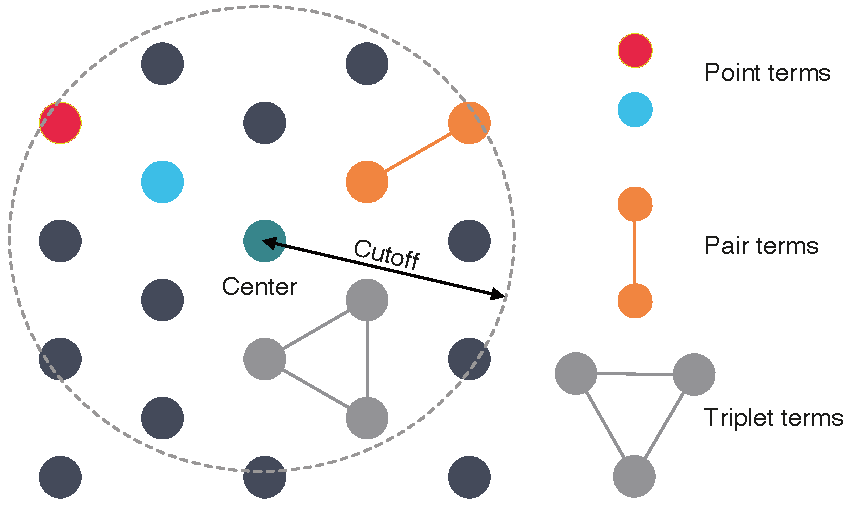
\includegraphics[width=1.0\columnwidth]{Figures/Cluster.pdf}
    \caption{Example of clusters that are typically encountered in a cluster expansion overlaid over a representative lattice. Within a cutoff distance from the center of a given lattice site, local orbits are drawn which extract the different interactions, such as point (red and blue dots), pair (orange dots), and triplet (grey dots). For each lattice, only the symmetrically-unique clusters are used to construct the cluster expansion.}
    \label{fig:lce}
\end{figure}

After determining $V_{\mathrm{orbit}}$ and $V_0$ in Eq.~\ref{eq:ekra_fit}, one  proceeds with kMC simulations, whose workflow is shown schematically in Fig.~\ref{fig:kmc}(a). In \texttt{kMCpy}, we have implemented the rf-kMC method, also known as the Bortz-Kalos-Lebowitz (BKL) algorithm \cite{bortz_new_1975}. Specifically, we list the set of all possible migration events in a given solid and their corresponding probabilities, amongst which one migration event is selected. Once a hop is selected, the hop is always executed, and subsequently, the list of possible migration events is updated. 

\begin{figure}[t]
    \centering
    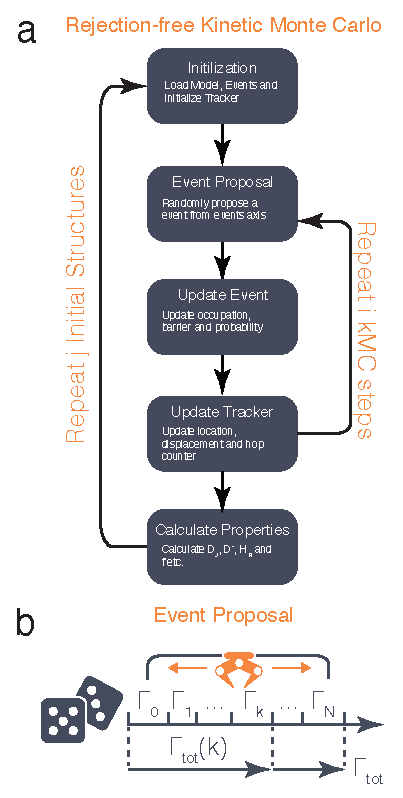
\includegraphics[width=0.8\columnwidth]{Figures/kmc.pdf}
    \caption{\textbf{a} Flow chart of the kMC process. $i$ kMC steps are repeated with each kMC simulation started from a different initial structure (i.e., $j$ initial structures in total).  \textbf{b} All migration events are listed on a hypothetical axis, with the solid line representing their hopping probabilities ($\Gamma$). An event no.\ $k$ is then randomly proposed based on a random number $\rho$. $\Gamma_\mathrm{tot}(k)$ is a cumulative sum of events from no.\ $0$ to no.\ $k$ (i.e., $\Gamma_{tot}(k)=\sum_{m=0}^k\Gamma_m$).  $\Gamma_{tot}$ is the sum of hopping probabilities of all migration events.}
    \label{fig:kmc}
\end{figure}

The typical procedure for the BKL method is summarized in the text below and in Fig.~\ref{fig:kmc}. Note that Fig.~{\ref{fig:kmc}} does not include the equilibration process.

\begin{enumerate}
    \item  \emph{Initialization}: In this step a representative structure is generated, which contains a fixed concentration of mobile ions and vacancies (assuming a vacancy-mediated migration mechanism). These structures can be obtained from canonical Monte Carlo (CMC), grand-canonical Monte Carlo (GCMC) \cite{xiao_understanding_2019} simulations, random structure generators \cite{evteev_shrinking_2008}, or  other structural enumeration techniques. During the initialization, a tracker is also set, which keeps track of the migration observables, such as, the mean squared displacement (MSD) of the diffusing species, the location of the center of mass, $D_J$, and $f$. 
    \item \emph{Event proposal}: A list of probabilities ($\Gamma_{m}$) is generated for all possible migrating paths ($m$) available for all mobile ions in the simulation box. This list also includes hops which may not be feasible. For example, if both the initial and final sites of a migration path are occupied by an atom (instead of one of the sites being vacant), the value of $\Gamma_{m}$ is set to 0. The hopping probability ($\Gamma$) for each migration event is calculated using the transition state theory \cite{vineyard_frequency_1957} via Eq.~\ref{eq:prob_hop}. 
    %
    \begin{equation}
    \label{eq:prob_hop}
    \Gamma = \nu^{*}  \exp \left(\frac{- E_{b}}{k_BT}\right)
    \end{equation}
    %
     From Eqs.~\ref{eq:ekra} and \ref{eq:ekra_fit}, it is possible to quickly generate $E_b$) for every possible hop. $\nu ^{*}$ is  the prefactor and is usually assumed to be of the order of $10^{11}$ to $10^{13}$~Hz \cite{van_der_ven_first-principles_2001,kaxiras_adatom_1994}. $T$ is the simulation temperature.   
    
    Following the generation of the probability list, a migration event ($k$) is chosen based on a random number (0~$< \rho <$~1), such that it satisfies Eq.~\ref{eq:choose_event}.
    %
    \begin{equation}
        \label{eq:choose_event}
        \frac{1}{\Gamma_\mathrm{tot}} \sum_{m=1}^{k-1} \Gamma_{m} < \rho \leq \frac{1}{\Gamma_\mathrm{tot}} \sum_{m=1}^{k} \Gamma_{m}
    \end{equation}
    %
    where $\Gamma_\mathrm{tot}$ is the sum of all the individual probabilities of all migration events. This step is shown schematically in Fig.~\ref{fig:kmc}(b).
    
    \item \emph{Update event and tracker}: After an event is chosen and executed, the time step ($\delta t$) is updated by drawing another random number (0~$< \zeta <$~1) as shown in Eq.~\ref{eq:timestep_update}.
    %
    \begin{equation}
        \label{eq:timestep_update}
        \delta t = - \frac{1}{\Gamma_\mathrm{tot}} \ln{\zeta}
    \end{equation}
    %
    Subsequently, the occupation vector, the new event list and their corresponding 
    probabilities, the displacement vector(s), the location(s) of the mobile ions, the location of the center of mass, and the hop counter are updated. 
\end{enumerate}

A single kMC pass includes repeating the event proposal, update event, and update tracker steps the same number of times as the number of mobile ions in the initialized structure. Generally, a large number of kMC passes are required to accurately predict transport properties. For example, Deng \textit{et al.}, undertook $\approx 10^{6}$ kMC passes to simulate Na-transport in  superionic conductor  over a millisecond scale \cite{deng_fundamental_2022}. After running a sufficiently large number of kMC passes, properties, such as, $D_J$, $D^{*}$, $H_R$, and $f$ are estimated. Thus, a collection of kMC passes for a single initial structure is referred to as a kMC run.  To get a better estimate of the transport properties at a given composition, \texttt{kMCpy} also calculates the properties as the initial structure is varied $j$ times (i.e., $j$ kMC runs). This ensures that the transport properties calculated represent the statistical estimate that is observed in experiments better.

%\hl{An in-depth understanding of the structure-property relationship of ion conductors at a given composition requires the repetition of the entire kMC simulations as the initial    conditions are varied.} This \hl{procedure is also required to establish} a statistical estimate of the \hl{computed} properties of the system and remove the bias of the observations from the initial structure.

\section{Overview of \texttt{kMCpy}}\label{sec:code}
\begin{figure*}
    \centering
    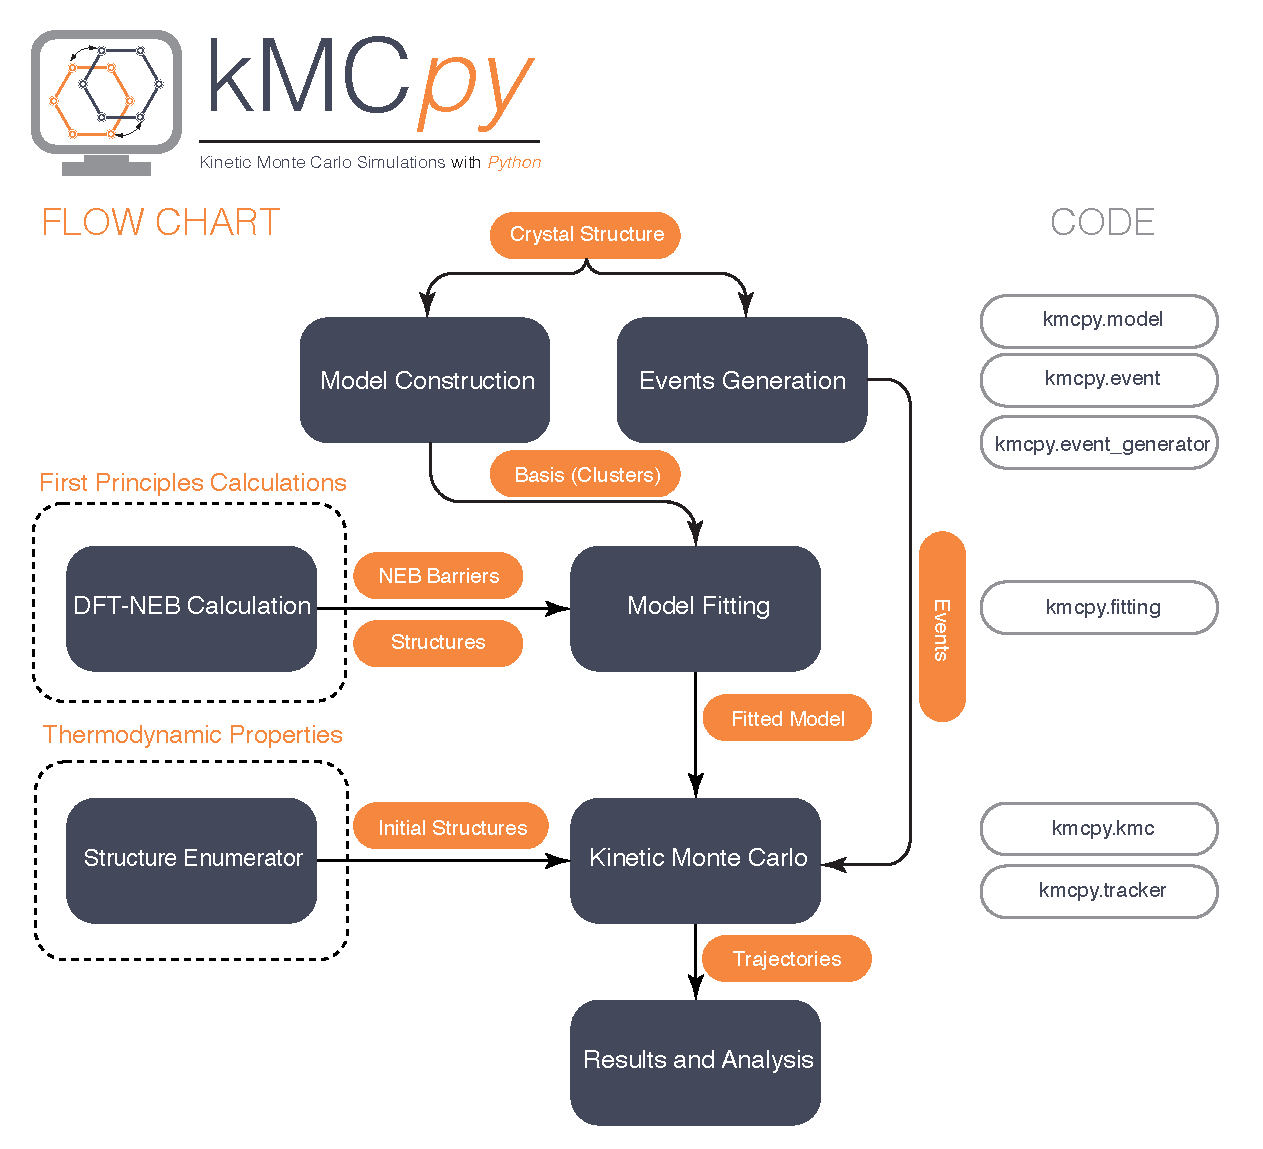
\includegraphics[width=1\textwidth]{Figures/Total_flowchart.pdf}
    \caption{\textbf{Left} Workflow of \texttt{kMCpy} package. \textbf{Right} \texttt{python} classes of \texttt{kMCpy} used for each stage of execution. Note that the initial structures for running kMC simulations are obtained from a structure enumerator. Migration barriers are computed from DFT-NEB calculations (dashed boxes). In the current version, only the LCE model has been implemented.}
    \label{fig:total_flowchart}
\end{figure*}

\subsection{Workflow}
\noindent The workflow of \texttt{kMCpy} is shown in Fig.~\ref{fig:total_flowchart}. The specific \texttt{python} classes for each action are shown as grey boxes on the right-hand side of Fig.~\ref{fig:total_flowchart}. \texttt{kMCpy} contains functions to analyse crystal structures, construct a LCE model and generate a list of possible migration events (see Sec.~\ref{sec:model} and \ref{sec:events}).  Starting from a list of DFT-NEB computed barriers, {\texttt{kMCpy}} fits a LCE model (see Sec.~{\ref{sec:fitting}}). The constructed model and events are then used to run kMC simulations with input structures from that are either the thermodynamic ground state(s) or any other user defined structures (Sec.~\ref{sec:kmc}). The trajectory of each mobile species are stored and analysed with a \texttt{Tracker} class as implemented in \texttt{kMCpy} (Sec.~\ref{sec:tracker}). Examples of input and output files are provided in Sec.~\ref{sec:io}. All \texttt{python} classes mentioned in the following sections can be stored in a human-readable JSON format and can be re-initialized after each stage. 

\subsection{Model Construction}\label{sec:model}
\noindent Before running a kMC simulation, a representative lattice model must be constructed to compute the barriers efficiently for any local environment, and the current version of \texttt{kMCpy} uses the LCE framework. However, the modular nature of \texttt{kMCpy} is such that other lattice models can also be used.

The LCE is implemented in the \texttt{LocalClusterExpansion} class in \texttt{\texttt{kMCpy}.model}. The local environment in the LCE model is described using a migration unit (\texttt{MigrationUnit}), which is defined as a representative collection of sites  centered around a given activated state (AS) where possible migration events can take place. The migration unit is generated using the user-specified cutoff radius. As a result, when a local environment is imported, an ``occupation vector'' (see Sec.~{\ref{sec:nomenclature}}) will be constructed based on the atomic species at each site.

Subsequently, all clusters within a migration unit are found by enumerating all points, pairs, triplets, etc.  via a cutoff radius (specified by the user) for each type of cluster.  All symmetrically equivalent clusters are then grouped as orbits, which become elements in the ``correlation vector'' (see Sec.~\ref{sec:nomenclature}). Clusters and orbits are coded into the \texttt{kMCpy.model} as the \texttt{Cluster} and the \texttt{Orbit} classes. In addition to the species and the atomic coordinates, \texttt{Cluster} and \texttt{Orbit} both have functions to compute ``correlation'' (see Sec.~\ref{sec:nomenclature}) for a given orbit based on the occupation of sites.

\subsection{Generating Events}\label{sec:events}
\noindent A kMC simulation needs a list of all possible migration events within a given simulation cell prior to its execution. Therefore, in \texttt{kMCpy}, we handle migration events using the \texttt{Event} class in \texttt{kmcpy.event}. \texttt{Event} stores the indices of two  sites (e.g., initial and final sites) involved in the migration event, as well as the indices of all sites within the surrounding migration unit, i.e., local environment indices. \texttt{Event} also has built-in functions to compute the correlation vector, the migration barrier and the hopping probability after an occupation vector has been assigned.

We enumerate all \texttt{Event} objects prior to the kMC run using a wrapper function,  \texttt{event\_generator.generate\_events()}, which receives the \texttt{LocalClusterExpansion} as input and loops through all migration units in the whole simulation cell to generate all possible events. From a given identifier of mobile species (i.e., the \texttt{mobile\_ion\_identifier} parameter), two sites indices involved in the migration event, namely, sites that the ion hops from and hops into, are identified. Subsequently, the indices of all sites in the current migration unit are stored for calculating the migration barrier.


\subsection{Model Fitting}\label{sec:fitting}
\noindent In order to fit DFT-NEB barriers using the LCE model, we have implemented the \texttt{Fitting} class in \texttt{kmcpy.fitting}. This function performs fitting by interfacing with the python package \texttt{scikit-learn}\cite{scikit-learn}. \texttt{kMCpy} also stores fitted results (i.e., the KECIs) in a portable JSON format. The current implementation of \texttt{kMCpy} uses the ``LASSO'' regression\cite{santosa_linear_1986}  to perform  fitting. Indeed, LASSO  limits the selection of orbits in the fit to the most important ones. LASSO requires a user-specified $\alpha$ parameter to reduce the total number of selected orbits. The \texttt{Fitting} class stores the fitting history, e.g. $\alpha$ and weights used during LASSO regression, for keeping a record and to fine tune the LCE. 

 Note that a LCE typically fits the $E_\mathrm{KRA}$ that is obtained from NEB calculations.  Therefore, the $\Delta E_\mathrm{end}$ term in Eq.~{\ref{eq:ekra}} can be computed either from CMC (e.g., by interfacing  other codes, such as "CASM" {\cite{thomas_casm_2022}}) or by fitting a separate LCE model. \texttt{kMCpy} has the flexibility to adopt either approaches to determine $E_\mathrm{end}$. In case a LCE is used for fitting $E_\mathrm{end}$ also, then the $E_\mathrm{end}$ data extracted from NEB calculations is used as an input for the fitting process.  

\begin{figure*}[!ht]
    \centering
    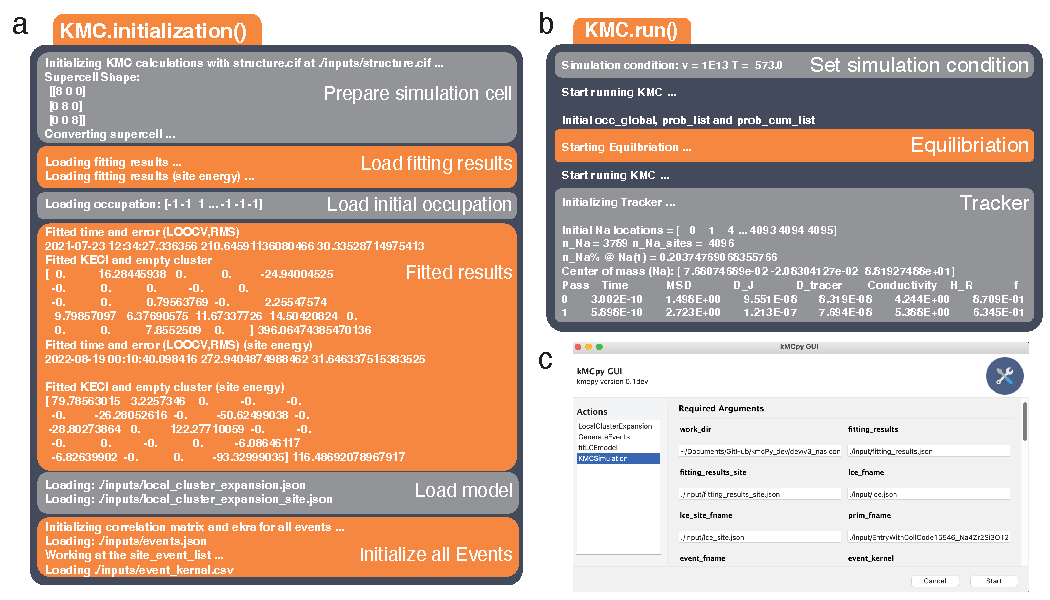
\includegraphics[width=1\textwidth]{Figures/output.pdf}
    \caption{Screenshots of initialization (\texttt{KMC.initialization()}, in {\bf a}) and  execution (\texttt{KMC.run()}, in {\bf b}) of kMC. \texttt{KMC.initialization()} prints the input parameters and \texttt{KMC.run()} shows the computed results. A \texttt{Tracker} object is intialized and subsequently called at the end of \texttt{KMC.run()}. {\bf c} shows the graphic user interface (GUI) of {\texttt{kMCpy}} relying on the \texttt{python} library {\texttt{Gooey}}.}  
    \label{fig:io}
\end{figure*}

\subsection{Kinetic Monte Carlo}\label{sec:kmc}
\noindent The \texttt{KMC} class in \texttt{kmcpy.kmc} can be used to perform kMC simulations. Multiple (e.g., 50) kMC runs should be done to eliminate the dependency of the results on the starting configurations. Initial structures of kMC runs are taken either from the thermodynamic ground state(s) (e.g., from CMC or GCMC simulations), or from a structure enumerator (see Fig.~\ref{fig:total_flowchart}). Auxiliary tools are provided in \texttt{kmcpy.tools.gather\_mc\_data} to extract occupation vectors from a structure in the crystallographic information file (CIF) format. 

The general process of rf-kMC is described in Fig.~\ref{fig:kmc}, and an example of a standard output of both the initialization and the execution processes of kMC is shown in Fig.~\ref{fig:io}a and b. The \texttt{KMC} class is firstly initialized using a size specification of the simulation (super)cell, the initial occupations, the fitted model, the generated events, and a reference crystal structure. When the LCE model is used, information about clusters, orbits, and the KECIs are provided. \texttt{kMCpy} then ``walks`` through all available migration events and evaluates the occupations, correlation vectors, and hopping frequencies, given a simulation temperature and a $\nu^{*}$. 

Upon initialization of the kMC, the \texttt{KMC.run()} function is called to perform the kMC simulation by supplying the total number of equilibration and sampling steps, respectively. The equilibration steps are not explicitly shown in Fig.~{\ref{fig:kmc}}a. A \texttt{Tracker} object is initialized once the equilibration process is complete (see Sec.~\ref{sec:tracker}). As shown in Fig.~\ref{fig:kmc}b, for each kMC step, an event $k$ is randomly proposed using \texttt{KMC.propose()}, based on Eq.~{\ref{eq:choose_event}}. 

After the proposed event is executed, the related occupations, correlations, and hopping frequencies are updated. Since a given site may be involved in multiple migration events, all events with sites associated with the proposed event are updated. The number of events that require updation after a proposed event is defined as the coupling strength of events, which can influence the computational performance of kMC (see Sec.~\ref{sec:performance}). We use a pre-computed table (\texttt{event\_kernel}) to quickly identify all events that need to be updated. 
    
\subsection{Tracking Diffusion}\label{sec:tracker}
\noindent To follow the displacements of all mobile species with respect to their original positions and to count the number of hops of each mobile ion, \texttt{kMCpy} uses a \texttt{Tracker} class in \texttt{kmcpy.tracker}.  This class is activated only after the equilibration is complete. The \texttt{Tracker} is initialized with the initial occupation vectors, a reference crystal structure of the simulation cell, the formal charge on migrating species, the dimensionality of the overall diffusion process, the average hopping distances (in $\Angstrom$), the simulation temperature, and $\nu^*$. The initial location of each migrating species is recorded and their displacement vectors and counters are set to zero during initialization. During each kMC step, \texttt{Tracker.update()} updates the displacement vector (taking into account periodic boundary conditions) and the hopping counter of the migrating species involved in a proposed event. 

Using Eqs.~{\ref{eq:jumpdiff}}-{\ref{eq:correlation_factor}} in Sec.~{\ref{sec:theory}}, \texttt{Tracker} computes transport properties, such as MSD, $D_J$, $D^*$, $\sigma$, $f$, and $H_R$ from the displacements of all migrating ions. The chemical diffusivity, $D_c$ (Eq.~\ref{eq:jumpdiff}) can be computed once $\Theta$ is identified for systems with variable compositions, such as electrodes \cite{van_der_ven_rechargeable_2020}. \texttt{Tracker.summary()} and \texttt{Tracker.write\_results()} routines  print and save the simulation results, respectively.

\subsection{Input and Output Files}\label{sec:io}
\noindent The inputs required by \texttt{kMCpy} (Fig.~\ref{fig:total_flowchart}a) can be prepared in JSON format, through the use of Jupyter notebooks for instance. Sample input files are provided in the \texttt{input\_example} folder of our Github repository (Footnote~\ref{fn:github}). Further, there is a command line wrapper to execute \texttt{kMCpy} from the command line, which can be found in \texttt{kmcpy.executable.wrapper}. Users can also customize their own workflow by importing specific modules, as described in the previous sub-sections.

An example of a standard output of \texttt{KMC.initialization()} and \texttt{KMC.run()} are shown in Fig.~\ref{fig:io}a and b. \texttt{kMCpy} prints the information imported from the JSON input files and sets the parameters described in Sec.~\ref{sec:kmc}, Sec.~\ref{sec:tracker}, and Fig.~\ref{fig:kmc}.

\texttt{kmcpy.executable.gui\_wrapper} offers a graphical user interface (GUI) as shown in Fig.~\ref{fig:io}c, which builds upon the \texttt{python} library \texttt{Gooey} \cite{kiel_gooey_2022}. This GUI covers all required and optional arguments for each step, providing a convenient way to test different parameters and for educational/demonstration purposes as well. 

A required task in the Actions box must be chosen in the GUI interface, in accordance to the descriptions in Sec.~\ref{sec:model} to Sec.~\ref{sec:kmc}. Next, all essential input parameters required for this task must be provided. For example, if \texttt{KMCSimulation} is chosen, one must provide: the work directory, the initial occupation, the original crystal structure, the fitted LCE model, the generated events, a value of $\nu^*$, and the simulation temperature. The  documentation is available via a website (\url{https://kmcpy.readthedocs.io}) with details on all input parameters to run \texttt{kMCpy} \cite{noauthor_kmcpy_2022}. By clicking the ``Start'' button, \texttt{kMCpy} will perform the selected task with the standard output of the simulation (similar to the command line output of Fig.~\ref{fig:io}a and b) displayed in a separate pop-up window.

\section{Performance of \texttt{kMCpy}}\label{sec:performance}
\noindent \texttt{kMCpy} has been developed in \texttt{python}, a high-level, human-interpretable language that combines flexibility and ease of programming. Since \texttt{python} is one of the most widely used programming languages\cite{perez_python_2011,noauthor_top_2022} both in the fields of materials informatics and data science, it provides a set of readily available tools and libraries that can be used to accelerate the development of new codes and libraries. Among them, we utilise a JIT compiler, \texttt{Numba} \cite{lam_numba_2015}, to increase the computational performance of \texttt{kMCpy}. Specifically, \texttt{Numba} translates the most numerically demanding part of \texttt{kMCpy} into optimized machine code. 

We emphasize that \texttt{kMCpy} is a serial code, i.e., a single kMC run is executed on a single CPU core. However, multiple kMC runs can be executed simultaneously on a multi-core platform, such as a high performance computing server or on the cloud. For example, different initial structures can be generated for a system and a kMC run for each initial structure can be run in parallel, thus reducing compute time.

Computationally, the intensive part of \texttt{kMCpy} is evaluating the correlation vector for each \texttt{Event}. Therefore, the size of the basis set (i.e., number of clusters and orbits), the total number events, and the coupling strengths between different events (see Sec.~\ref{sec:nomenclature}) can crucially influence the determination of the  correlation vector  and the computational performance. For example, the basis-set size controls the computational cost of updating the correlation vector of a single event, whereas the total number of unique events and the coupling strengths between events set the total number of events to be updated during each kMC step. These quantities are usually coupled with each other, i.e., larger cutoff radii usually lead to larger basis sets, and in turn, stronger coupling between events, resulting in an increased computational cost of the kMC run.

We benchmarked\footnote{All benchmarks were performed on a 2020-year model 13-inch Apple MacBook Pro with  a M1 chipset (8 core CPU + 8 core GPU) and 16 GB of RAM.\label{fn:hardware}} the computational performance of \texttt{kMCpy}, with the data compiled in Table~\ref{tab:performante}, which shows the time required to prepare inputs and run a very short simulation on a test system\footnote{A LCE model for Na ion migration was built with a $\sim$6~\AA{} cutoff radius for point, pair and triplet clusters on \ce{Na_{1+x}Zr_2P_x Si_{3-x}O_{12}}, yielding a total of 19 unique orbits and 212 possible clusters. The LCE model was fitted with data from DFT-NEB calculations. 6144 Na-ion hopping events were generated in a $8\times8\times8$ supercell lattice\label{fn:model_details}.}.  The process of input preparation includes construction of the model, fitting of the model, and events generation, which in total takes less than 10s. 100 kMC passes (51,200 steps per pass) on this model takes $\sim$3 minutes, indicating that the time required for preparing the input is generally marginal compared to the kMC simulation itself. 

\begin{figure*}[!ht]
    \centering
    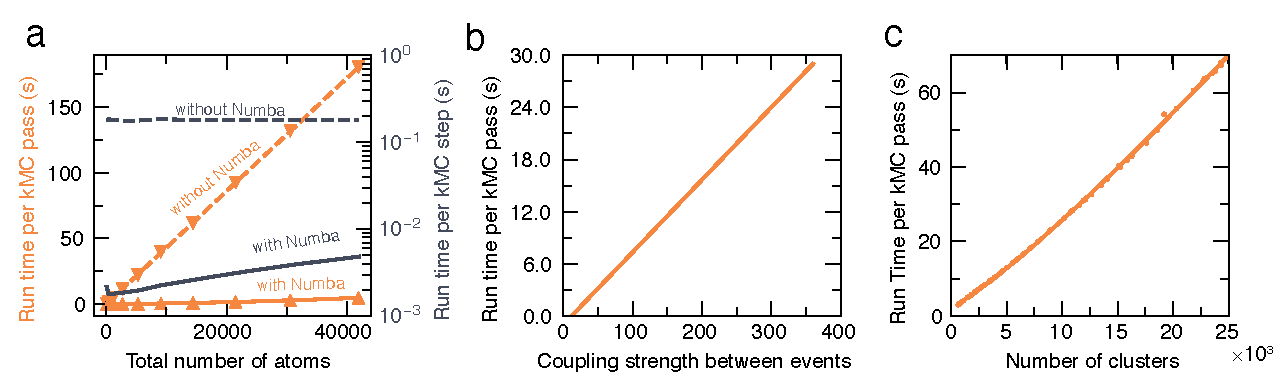
\includegraphics[width=1\textwidth]{Figures/scalability.pdf}
    \caption{{\bf a} shows the average computing time, per kMC pass (left y-axis, orange lines) and per kMC step (right y-axis, black lines), as a function of total number of atoms for kMC simulations of \ce{Na_{1+x}Zr_2P_x Si_{3-x}O_{12}}, scaling from $1\times1\times1$ (42 atoms) to $10\times10\times10$ supercells (42,000 atoms). The details of this model can be found in Ref.~\cite{deng_fundamental_2022}. Solid and dashed lines refers to the time consumption with and without \texttt{Numba}, respectively. The LCE model contains 19 unique orbits and 212 possible clusters, with a coupling strength of 12.  \textbf{b} shows the relationship between the time consumption and coupling strength between events (defined in Section~\ref{sec:nomenclature}) performed on a $8\times8\times8$ supercell lattice.  \textbf{c} describes the effect of basis set size (number of clusters/orbits in LCE model) on simulation time, using the $8\times8\times8$ supercell.}   
    \label{fig:performance}
\end{figure*}

Eq.~{\ref{eq:performance}} shows fitted dependencies between the simulation time and the three major factors:
%
\begin{equation}
t\propto f_\mathrm{Numba}(N_\mathrm{cell})\times {N}_\mathrm{cluster}^{1.16}\times N^{1.01}_\mathrm{cell} \times {N^{1.10}_\mathrm{coupling}}
  \label{eq:performance}
\end{equation}
%
where $N_\mathrm{cluster}$, $N_\mathrm{cell}$, $N_\mathrm{coupling}$ are the number of clusters, size of the supercell, and the coupling strength, respectively. $f_\mathrm{Numba}$ denotes the acceleration effect  using the  \texttt{Numba} routines on the computational time. The benchmark results are shown in Fig.~\ref{fig:performance}. 

The average simulation time using different cell sizes (indicated by total number of atoms per simulation box) is depicted in Fig.~\ref{fig:performance}a. Without \texttt{Numba}, the elapsed time  per kMC step remains approximately constant $\sim 10^{-1}$~s (dashed black line). \texttt{Numba} accelerates significantly the kMC simulation by factor of $\sim$2 ($10^{-3}$~s, solid black line). The speedup by {\texttt{Numba}}} is weakened when the simulation cell becomes larger. Therefore,  {\texttt{Numba}} can enable access to longer and larger scale simulations with \texttt{kMCpy} \cite{deng_fundamental_2022}.  As 1 kMC pass is just the total number of available sites within the simulation cell, the run time per kMC pass grows linearly when the cell size (i.e., number of atoms) become larger. Fig.~\ref{fig:performance}b and c demonstrate the effect of the coupling strength between events as well as the basis set size, which also contribute a quasi-linear increase towards the run time per kMC pass. These results show that the time complexity of the implemented kMC algorithm is $O(\sim N)$.

\begin{table}[!h]
    \centering
    \caption{Time (in s) distribution for bootstrapping and running a kMC simulation of a test model. Details of hardware information and input model to perform these benchmarks are mentioned in Footnotes~\ref{fn:hardware} and \ref{fn:model_details}.}
    \begin{tabular}{lr}
    \hline
        Action & Time Spent (s) \\ \hline
        Model Generation (212 clusters) & 2.1 \\ 
        Model Fitting (19 orbits) & 2.6 \\ 
        Events Generation (6,144 events) & 1.31 \\ 
        kMC simulation (100 passes/51,200 steps) & 168 \\ \hline
    \end{tabular}
    \label{tab:performante}
\end{table}


\section{Conclusion}\label{sec:conclusion}
\noindent In summary, we presented \texttt{kMCpy},  a light-weight open-source \texttt{python} package  to perform kMC simulations of ionic transport in crystalline solids, with inputs from DFT calculations. \texttt{kMCpy} and its implemented workflow provide a framework to the scientific community to predict transport properties of any crystalline solid with high accuracy and performance. The design of \texttt{kMCpy} should facilitate its use on most available computational platforms from standard laptops to high performance supercomputers. The modular framework makes it highly customizable and easily programmable. By utilizing the JIT compiler -- \texttt{Numba}, \texttt{kMCpy} achieves high computational performance. Both the input and the output files of \texttt{kMCpy} rely on the human-readable JSON format, which is easy to distribute. Future developments of \texttt{kMCpy} include: i) utilizing GPU-based acceleration for better performance, ii) developing a thermodynamic (CMC/GCMC) module and a structure enumerator, and iii) adding additional models for the evaluation of $E_{\mathrm{KRA}}$ that are alternative to LCE. 

\appendix
\section{Nomenclature}\label{sec:nomenclature}
\begin{itemize}
    \item \textbf{Site}: $i \in \{0,1,...,N-1\}$ is a site in a simulation cell with $N$ sites. $i$ is a unique global index of a site.

    \item \textbf{Occupation}: in a Chebyshev basis $\sigma_i$ has a value of $\pm$1  for site $i$, e.g., occupied ($-1$) or unoccupied ($+1$), or species A ($-1$) and species B ($+1$).

    \item \textbf{Occupation Vector}: $\vec{\sigma}=[ \sigma_0,\sigma_1,...\sigma_{N-1}]$ is a vector of occupations in a simulation cell.
    
    \item \textbf{Migration unit}: $M=[i_0,i_1,...,i_m]$ is a collection of all sites within a specific cutoff radii around the centre of a migration unit, where $m$ is the total number of sites within that migration unit. There are multiple migration units in the simulation cell.
    
    \item \textbf{Sublattice Site}: $i \in \{0,1,...,n-1\}$ is a site within a migration unit with $n$ sites.

    \item \textbf{Distance Matrix: D}: Distance matrix of a migration unit is a $m\times m$ matrix where $m$ has been defined above. Matrix elements $d_{ij}$ are the Cartesian distances between site $i$ and $j$ within a migration unit.

    \item \textbf{Cluster}: $[i_0,i_1,...i_{n}]$ is a collection of sublattice sites ($i$) within a migration unit with a length of $n$. Presently there are four types of cluster implemented in the code:

    Point: a cluster containing 1 site, $n=1$;
    
    Pair: a cluster containing 2 sites, $n=2$;
    
    Triplet: a cluster containing 3 sites, $n=3$;
    
    Quadruplet: a cluster containing 4 sites, $n=4$;
    
    Note, the order-size of these clusters can be easily extended beyond 4.
    \item \textbf{Cluster Function}: $\phi_{\alpha}(\vec{\sigma})=\prod_{i \in \alpha}\sigma_i$ is a product of all occupations of all sites that belong to a cluster.

    \item \textbf{Orbit}, $[\alpha[0],\alpha[1],...\alpha[m]]$ is a collection of symmetrically equivalent clusters with a multiplicity of $m$ within a migration unit.

    \item \textbf{Correlation}: $\phi_{O}(\vec{\sigma})=\sum_{\alpha\in O}\phi_{\alpha}(\vec{\sigma})$ is the summation of cluster functions of all symmetrically equivalent clusters within a migration unit that belongs to an orbit.
    
    \item \textbf{Correlation Vector}:
    \begin{equation}
    \vec{\phi}(\vec{\sigma})=[\phi_{O[0]}(\vec{\sigma}),\phi_{O[1]}(\vec{\sigma}),...,\phi_{O[n]}(\vec{\sigma})]
    \end{equation} is a collection of all correlations for each orbit within a migration unit with a length of $n$. This is also the basis-set size.

    \item \textbf{Cluster Expansion Model}: 
    \begin{equation}
        E(\vec{\sigma})=V_0+\sum_{\alpha} V_{\alpha} \phi_{\alpha}(\vec{\sigma})
    \end{equation} 
    where $E$ is total energy (typically the DFT total energy,  and $V_0$ and $V_{\alpha}$ are called effective cluster interactions (ECIs) for each cluster, which are fitted from first-principles calculations. The summation polynomials are usually truncated to specific cluster size (e.g., quadruplet, quintuplet). All  clusters belong to the same orbit shares the same $V_{\alpha}$.
    
    \item \textbf{Local Cluster Expansion Model} uses a local  cluster expansion model,
    %
    \begin{equation}
        E_\mathrm{KRA}(\vec{\sigma})=K_0+\sum_{\alpha} K_{\alpha} \phi_{\alpha}(\vec{\sigma})
        \label{eq:CE}
    \end{equation}
    %
    where $E_\mathrm{KRA}$ is  the kinetic resolved activation energy barrier which is independent of migration directions. $K_0$ and $K_{\alpha}$ are called kinetic effective cluster interactions (KECIs), which are fitted from first-principles NEB calculations. The directional dependent activation energy can further be recovered using 
    %
    \begin{equation}
    E_{b} = E_\mathrm{KRA}(\vec{\sigma}_{AS}) + \frac{1}{2}\Delta E_\mathrm{end}
    \end{equation}
    %
    where $\vec{\sigma}_{AS}$ is the occupation vector at the activated state and $E_b$ is the activation energy barrier from initial to final images. $\Delta E_\mathrm{end}$ is the total energy difference between the final and initial images, respectively:
    %
    \begin{equation}
        \Delta E_\mathrm{end} =E(\vec{\sigma}_\mathrm{final}) - E(\vec{\sigma}_\mathrm{initial})
    \end{equation}
    %
    \item \textbf{Event} is a swap of occupation values between two hopping sites.
    
    \item \textbf{Pass} is defined as the total number of mutable sites in the simulation cell.
    
    \item \textbf{Coupling Strength Between Events} is the total number of events that need to be updated after an event has been executed.
\end{itemize}

% \subsection{Sorting of sublattice index}\label{sec:distance_matrix}
% \wx{I believe that this paragraph need to be improved. Please comment, and also we shall decide if we really want to keep this paragraph}

% In kMCpy, events correspond to possible hopping between two sites. The energy/probability of such hopping is related to the \(E_{KRA}\) calculated from the occupation of sites in the migration unit defined in the local cluster expansion. Therefore, we need following information to generate event:

% 1. the site index, of which the mobile ion hop from

% 2. the site index, of which the mobile ion hop to

% 3. m site indices of all sites in the migration unit that involved in the \(E_{KRA}\) calculation

% 4. Hamiltonian of local cluster expansion correspond to the sites in migration unit.

% Here we propose a distance matrix method to accelerate the generating process, which avoid repeating identification of Hamiltonian. The first migration unit \(\mathbf{M}_0\) is termed as reference migration unit. Sites of reference migration unit are first grouped by their specie, then in each group the sites are sorted by its x coordinate (if x coordinate the same, then by random). Such operation yield a unique sequence of the reference migration unit \(\mathbf{M}'_0\). We represent this sorting as a mapping \(f_0\). 

% \(f_0:\mathbf{M}_0={\{i_0,i_1,...i_{m}\}}->\mathbf{M}_0'={\{i'_0,i'_1,...i'_{m}\}}\) 

% Given a well converged local cluster expansion model, i.e., property of cluster is well defined. We then identify every clusters according to the specie and distance information from \(\mathbf{M}_0'\), and establish the Hamiltonian, i.e., relationship between occupation vector \(\vec{O_0}\) of \(\mathbf{M}'_0\), and diffusion barrier \(E_{KRA}\).

% \(E_{KRA}={\hat{\mathcal{H}}}^0_{cluster}\vec{O_0}= {\hat{\mathcal{H}}}^0_{point} \cdot \vec{O_0}  +\frac{1}{2}{\hat{\mathcal{H}}}^0_{pair}:(\vec{O_0}\otimes \vec{O_0}) +\frac{1}{6}{\hat{\mathcal{H}}}^0_{triplet}\vdots(\vec{O_0}\otimes \vec{O_0}\otimes \vec{O_0})+....\)

% Here \(\vec{O}\) and \({\hat{\mathcal{H}}}_{point}\) is a vector, \((\vec{O}\otimes \vec{O})\) and \({\hat{\mathcal{H}}}_{pair}\) is a matrix, and \((\vec{O}\otimes \vec{O}\otimes \vec{O})\) is a tensor. \(\cdot : \vdots\) are dot product, frobenius product, tensor inner product respectively.

% Based on the sequence \(\mathbf{M}'_0\), a \(m\times m\) reference distance matrix \(\mathcal{D}_0\) is built (m equals to the number of sites in migration unit) with the element \(d_{jk}\) being the cartesian distance between jth element and kth element of sequence \(\mathbf{M}_0'\). 

% %
% \begin{equation}
%   \mathrm{\mathcal{D}_0=\begin{bmatrix}
%  d_{i'_0,i'_0}      &  d_{i'_1,i'_0}     &  d_{i'_2,i'_0}     & \cdots   &  d_{i'_m,i'_0} \\
% d_{i'_0,i'_1}      &  d_{i'_1,i'_1}     &  d_{i'_2,i'_1}     & \cdots   &  d_{i'_m,i'_1} \\
% d_{i'_0,i'_2}       & d_{i'_1,i'_2}    &  d_{i'_2,i'_2}   & \cdots     &  d_{i'_m,i'_2} \\
%  \vdots & \vdots & \ddots &        &  \vdots \\
%  \vdots & \vdots &        & \ddots &  \vdots\\
% d_{i'_0,i'_m}       & d_{i'_1,i'_m}           &  d_{i'_2,i'_m}   & \cdots     &  d_{i'_m,i'_m} 
% \end{bmatrix}
% }  
%   \label{eq:distancematrix}
% \end{equation}
% %

% Event generator shall loop through all migration unit in order to generate events. In the next migration unit, again the sites are grouped by their specie. Then instead of sorting by x coordinate, the sequence of sites in each specie group is enumerated until there is a sequence of which the corresponding distance matrix \(\mathcal{D}_1\)is the same (or within sufficiently small tolerance considering error from float point numbers) as the reference distance matrix \(\mathcal{D}_0\). We represent the new sorting as a mapping \(f_1\) (This mapping is not necessarily unique, and depends on the symmetry of migration unit)

% \(f_1:\mathbf{M}_1={\{i_0^1,i_1^1,...i_{m}^1\}}->\mathbf{M}_1'={\{i^1_0',i_1^1',...i^1_{m}'\}}\)

% For \(\mathbf{M}_1'\), the Hamiltonian \({\hat{\mathcal{H}}}_1\) is the same as \({\hat{\mathcal{H}}}_0\) due to the following reason:

% Each single site in the migration unit forms a point cluster, and the type of point cluster \(\alpha_i\) is fully identified by the type of species \(Z_i\). The specie of jth site in \(\mathbf{M}'_0\) is the same as the jth site in \(\mathbf{M}_1'\) as we group them by species. Therefore jth site in \(\mathbf{M}'_0\) is the same point cluster as jth site in \(\mathbf{M}_1'\)

% For every two sites in the migration unit, they form a pair cluster \(\alpha_{ij}\) and type of the pair cluster can be determined by the type of specie of two sites \(Z_i. Z_j\)and their distance \(d_{ij}\). For pair cluster formed by jth and kth site in \(\mathbf{M}'_0\), the species are the same as jth and kth site in \(\mathbf{M}'_1\). The distance between jth and kth site is also the same in two migration unit if the distance matrix are the same. \(D^0_{jk}=D^1_{jk}\). Therefore jth and kth site in \(\mathbf{M}'_0\) form the same pair cluster as jth and kth site in \(\mathbf{M}'_1\)

% Similar for triplet and quadruplet cluster.

% The distance matrix method therefore eliminate the labour of repeating identification of cluster or Hamiltonian, and increase the speed of generating events from \(O(m^4)\) (identifying quadruplet cluster) to \(O(m^2)\) (for generating a 2D distance matrix).
\subsection*{Acknowledgment}
\noindent We acknowledge funding
from the National Research Foundation under his NRF Fellowship
NRFF12-2020-0012. The
computational work was performed on resources of the National
Supercomputing Centre, Singapore (\url{https://www.nscc.sg}). 


% To print the credit authorship contribution details
\printcredits

%% Loading bibliography style file
%\bibliographystyle{model1-num-names}
% \bibliographystyle{cas-model2-names}
% \bibliographystyle{model-num-names}
\bibliographystyle{elsarticle-num}
% Loading bibliography database
\bibliography{kmcpy_ref}
%
%% Biography
%\bio{}
%% Here goes the biography details.
%\endbio
%
%\bio{pic1}
%% Here goes the biography details.
%\endbio

\end{document}

